% Section: sequential (\input from main.tex)
\section{A* in the Sequential World}
\label{sec:seq}

\subsection{Implementation}

\texttt{astar()} is the textbook algorithm. OPEN is a binary heap of
$(f, v)$ pairs with lazy deletion: instead of decreasing a key, a node is
pushed again and outdated entries are skipped when popped. $g$-values and
parent pointers are arrays indexed by node. The function is a template over
the heuristic and the edge-weight functor, so the same code serves every
variant in this section, including the dynamic ones:

\begin{lstlisting}
while (!open.empty()) {
  auto [f, u] = open.top(); open.pop();
  if (closed[u]) continue;                                   // duplicate entry
  if (H::dynamic) {                                          // h may have changed
    Cost fnow = g[u] + h(u);
    if (fnow > f && !open.empty() && fnow > open.top().first) {
      open.push({fnow, u}); continue;                        // lazy re-keying
    }
  } else if (f > g[u] + h(u)) continue;                      // outdated entry
  closed[u] = 1; h.tick();
  if (u == t) break;
  for (auto e = G.begin(u); e != G.end(u); ++e) {
    Cost ng = g[u] + W(*e);
    if (ng < g[e->to]) {
      if (closed[e->to]) closed[e->to] = 0;                  // re-open
      g[e->to] = ng; parent[e->to] = u; open.push({ng + h(e->to), e->to});
    }
  }
}
\end{lstlisting}

\paragraph{Heuristic.} The default $h$ is the great-circle (haversine) distance
to the target. For the time metric it is divided by $v_{\max}$, the highest
speed that occurs anywhere in the graph. Edge costs are rounded \emph{up} to
whole millimetres or milliseconds and $h$ is rounded \emph{down}, so $h$ is
admissible and consistent by construction; Section~\ref{sec:seq-test} checks
this on every edge. A consistent $h$ never re-opens a closed node, so the
re-opening branch above is needed only for the heuristics of
Section~\ref{sec:seq-dyn}.

% Subsection: review of the lecture material (\input from sections/sequential.tex)
\subsection{Checking the lecture's pseudocode and reference notebook}
\label{sec:review}

The lecture slides ask to ``check the correctness of the left algorithm'' (the
A* pseudocode on slides 9--10), and the reference notebook
\texttt{osm-astar.ipynb} is marked ``not yet verified''. We checked both.

\paragraph{Pseudocode (slides 9--10).}
\begin{itemize}[nosep]
  \item The selected vertex $u$ is added to $C$ but \textbf{never removed from
        $O$}. The next iteration selects the same $u$ again, so the loop never
        progresses. The fix is $O := O \setminus \{u\}$ after the selection.
  \item Neighbours already in $C$ are skipped. This is correct only for a
        \emph{consistent} $h$. With a dynamic or uncertain $h$ (the question on
        slide~10) a closed vertex can later be reached with a smaller
        $g$, and it must be re-opened (Section~\ref{sec:seq-dyn}).
  \item When $O$ becomes empty without reaching $d$, the procedure ends
        without reporting that no path exists.
\end{itemize}

\paragraph{Reference notebook.} We ran the notebook's
\texttt{astar\_shortest\_path} unchanged on our graph, loaded as an OSMnx-style
\texttt{MultiDiGraph}, and compared it with \texttt{networkx} shortest paths.
Table~\ref{tab:review} lists what we found. The most serious problem is B9: in
an OSMnx \texttt{MultiDiGraph}, \texttt{graph[u]} maps each neighbour to a
dictionary of \emph{parallel edges} (\texttt{\{0: \{'length': ...\}\}}), so
\texttt{edge\_data.get('length', 1)} always returns the default 1. Every road
segment then costs 1\,m, and the code minimises the number of segments. This
explains the weight printed in the notebook: 0.34\,min for a trip across the
city. On our graph the same example is a 19.1\,km route that takes 41\,min with
the lecturer's speed profile.

\begin{table}[H]
\centering
\small
\caption{Problems found in \texttt{astar\_shortest\_path} of the reference
notebook, measured with the code unchanged on 60 random queries on our city
graph.}
\label{tab:review}
\begin{tabularx}{\linewidth}{l >{\raggedright\arraybackslash}p{4.6cm} Y}
\toprule
 & \textbf{Problem} & \textbf{Effect and fix} \\
\midrule
B1 & \texttt{f\_score\_neighbor = g\_score + h\_score} uses the \emph{current} node's $g$ and $h$ & the queue is not ordered by the neighbour's $f$, so the search is not A*. Fix: $g_{\mathrm{nb}} + h_{\mathrm{nb}}$ \\
B2 & \texttt{t = t + ...} inside the neighbour loop & the current node's clock grows with every neighbour scanned. Fix: a separate $t_{\mathrm{nb}}$ \\
B3 & \texttt{speeds[floor(t)]}, $t$ in minutes, 20 slots & \texttt{IndexError} for trips longer than 20\,min; hidden only by B9 (with B9 fixed, the code crashes). Fix: cyclic profile \\
B4 & Euclidean distance on longitude/latitude \emph{degrees} & $h \approx 10^{-4}$\,min: the search expands as many nodes as Dijkstra (198\,718 against 198\,722 on a long query). Fix: great-circle distance in metres \\
B5 & $h = d / \textit{speed}(t)$ & over-estimates when later slots are faster, so $h$ is not admissible (Section~\ref{sec:seq-td}). Fix: $d / v_{\max}$ \\
B6 & \texttt{shortest\_path\_at\_time} runs a full Dijkstra in every call of $h$ & 0.6\,s per generated node on the city graph; not admissible either (B5). Fix: one reverse Dijkstra per destination \\
B7 & edge time uses only the speed at departure & not FIFO: 6.3\% of random (departure, length) pairs arrive earlier when leaving later, so label-setting A* is not exact. Fix: integrate the speed over the slots \\
B8 & the whole path is copied into every queue entry; no best-$g$ check & $O(\text{path length})$ memory per entry and many useless duplicates. Fix: parent array \\
B9 & \texttt{edge\_data.get('length', 1)} on a \texttt{MultiDiGraph} & always 1: routes are 26\% longer than the shortest route on average (up to $2.2\times$), and the reported weight is 0.48\,min instead of 37.8\,min. Fix: minimum over parallel edges \\
B10 & returns \texttt{f\_score} as the path weight & wrong whenever B1 applies. Fix: return the arrival time minus the departure time \\
\bottomrule
\end{tabularx}
\end{table}

The corrected notebook (\texttt{notebooks/osm-astar-fixed.ipynb}) keeps the
original function next to the fixed one. On 60 random queries with four
departure times, the fixed time-dependent A* returns exactly the travel time
of an independent oracle and of the uninformed search
(Section~\ref{sec:seq-td}). Our C++ implementation follows the same
corrections.


\subsection{Dynamic and uncertain heuristic}
\label{sec:seq-dyn}

In a live navigation system the remaining cost comes from a predictor that is
noisy and changes while the search runs. We model both effects:

\begin{itemize}[nosep]
  \item \textbf{Uncertain $h$:} $h(v) = h_0(v)\,(1 + \varepsilon U)$ with
        $U \sim \mathcal{U}(-1, 1)$ drawn \emph{at every evaluation}. Two
        evaluations of the same node can return different values, like a
        noisy sensor.
  \item \textbf{Dynamic $h$:} $h_k(v) = h_0(v)\,\lambda(k)$ with
        $\lambda(k) = 1 + \varepsilon \sin(2\pi k/300)$, where $k$ is the
        number of expansions so far. This is a traffic forecast that is
        refreshed periodically during the search.
\end{itemize}

Both heuristics break the assumptions of textbook A* in three ways, and the
code handles each of them:

\begin{enumerate}[nosep]
  \item $h$ is no longer consistent and can over-estimate by up to a factor
        $1+\varepsilon$. A node can then be reached later with a smaller $g$,
        so closed nodes must be \textbf{re-opened}.
  \item The key stored in OPEN becomes \textbf{stale} when $h$ changes. On
        every pop the key is recomputed with the current $h$. If it is now
        larger than the next key in the heap, the node is pushed back instead
        of being expanded (lazy re-keying).
  \item The returned cost is recomputed along the final parent chain, because
        a re-opened ancestor may have improved after the goal was reached.
\end{enumerate}

Since $h \le (1+\varepsilon)\,h^*$ for every evaluation, the usual
weighted-A* argument bounds the result: $C^* \le C \le (1+\varepsilon)\,C^*$.

% Subsection: time-dependent travel times (\input from sections/sequential.tex)
\subsection{Time-dependent travel times (the lecturer's model)}
\label{sec:seq-td}

The reference notebook makes $h$ dynamic in a concrete way: the speed changes
with the time of day. A profile of 20 slots gives one network-wide speed per
slot (350--600\,m/min), and a trip that departs at time $t$ drives at
$\mathit{speeds}[\lfloor t \rfloor]$. Both the travel time of an edge and the
heuristic then depend on the time at which a node is reached. We implemented
this model in C++ (\texttt{td\_astar}, \texttt{SpeedProfile}) with three
corrections to the notebook (Section~\ref{sec:review}):

\begin{enumerate}[nosep]
  \item \textbf{FIFO edge times.} The time to drive an edge integrates the
        speed over every slot the edge spans. Leaving later can then never
        mean arriving earlier, which is the condition under which
        label-setting A* (and Dijkstra) remain exact for time-dependent costs.
        Using only the speed at departure, as the notebook does, violates this
        for 6.3\% of random (departure time, length) pairs.
  \item \textbf{Admissible heuristic.} $h(v) = d_{\mathrm{gc}}(v,t)/v_{\max}$,
        where $d_{\mathrm{gc}}$ is the great-circle distance and $v_{\max}$ the
        highest speed of the profile, never over-estimates, whatever the time.
        The notebook divides by the speed at the current time, which
        over-estimates whenever faster slots follow.
  \item \textbf{Cyclic profile,} so that trips longer than 20 slots stay
        inside the array.
\end{enumerate}

\paragraph{Testing.} Test T6 checks FIFO on 200\,000 random pairs, and runs
100 random queries at random departure times. Because the speed is the same on
every road at a given moment and travel is FIFO, the fastest route is the
shortest-length route, and its travel time is $\mathrm{arrive}(t_0, L^*) - t_0$.
This gives an oracle that does not share code with A*. Time-dependent A* and
time-dependent Dijkstra must both match it to $10^{-6}$\,min; they do on all
five platforms.

\begin{table}[H]
\centering
\small
\caption{Part 1: time-dependent A* with the lecturer's speed profile; 200
queries $\times$ 4 departure times. Expanded, re-opened and quality
(cost/optimum) are from Platform~C; B and C use the same queries. The road
distance $d_{\mathrm{road}}$ needs one reverse Dijkstra per destination, which
is not included in the time.}
\label{tab:td}
\begin{tabular}{l rrrrr r}
\toprule
Heuristic & ms (A) & ms (C) & expanded & re-opened & mean & worst \\
\midrule
$h = 0$ (time-dependent Dijkstra) & 6.6 & 19.8 & 104{,}414 & 0 & 1.000 & 1.000 \\
$h = d_{\mathrm{gc}} / v_{\max}$ & 4.3 & 12.8 & 44{,}367 & 0 & 1.000 & 1.000 \\
$h = d_{\mathrm{road}} / v_{\max}$ (one reverse Dijkstra) & 2.0 & 5.7 & 25{,}439 & 0 & 1.000 & 1.000 \\
$h = d_{\mathrm{gc}} / \mathit{speed}(t)$ (lecturer) & 4.5 & 16.2 & 62{,}804 & 45{,}665 & 1.045 & 1.288 \\
\bottomrule
\end{tabular}

\end{table}

\begin{figure}[H]
\centering
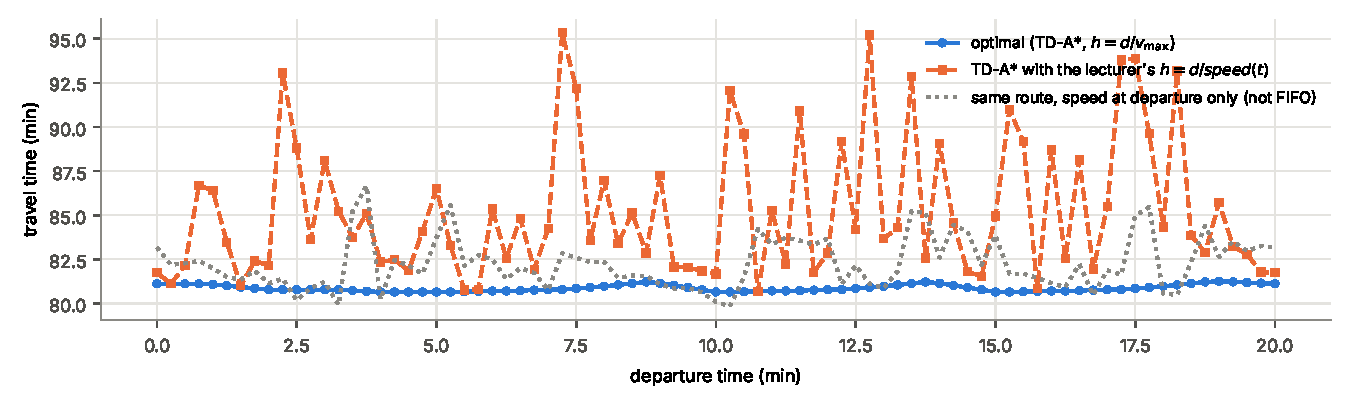
\includegraphics[width=\linewidth]{figures/fig9_td.pdf}
\caption{Part 1: travel time of the longest of the 200 queries as a function
of the departure time (Platform~C).}
\label{fig:td}
\end{figure}

\textbf{The lecturer's heuristic is not admissible, and it shows.} With
$h = d/\mathit{speed}(t)$, 87\% of the 800 runs return a route that is slower
than the optimum, by 4.5\% on average and by up to 29\%. Because the
estimate jumps whenever the clock crosses a slot boundary, the search also
re-opens 45\,665 nodes per query. It is not even faster: it expands more nodes
than the admissible great-circle heuristic (62\,804 against 44\,367).
Figure~\ref{fig:td} shows the same effect for one long trip: the optimal
travel time varies by only 0.6\,min with the departure time, while the
lecturer's heuristic adds up to 14.5\,min. The non-FIFO edge model of the
notebook gives yet another travel time, between 0.9\,min less and 6.0\,min more than the
correct one, because it charges the whole edge at the speed of the slot in which the
car enters it.

\textbf{A better admissible heuristic pays off.} The road distance to the
target divided by $v_{\max}$ is still admissible but much tighter: it needs
43\% fewer expansions than the great-circle heuristic (25\,439 against 44\,367) and is
3.3--3.5$\times$ faster than time-dependent Dijkstra. This is the correct version
of the notebook's \texttt{shortest\_path\_at\_time} idea: compute the road
distances once per destination with a reverse Dijkstra, instead of one full
search per evaluation of $h$.


\subsection{\texorpdfstring{Vector-valued $f$}{Vector-valued f}: multi-objective A*}

With a vector-valued $f$ there is no single optimum. The goal becomes the set
of \textbf{Pareto-optimal} routes, i.e.\ routes that no other route beats in
every objective. We minimise \textbf{(length, congested travel time)}. The two
objectives conflict: short routes use small streets, fast routes use main roads
that are congested at rush hour.

We implement \NAMOA{}~[3]. The scalar $g(v)$ becomes two sets of
non-dominated cost vectors per node, $G_{op}(v)$ and $G_{cl}(v)$. A new label
$(g, v)$ is generated only if no label already stored at $v$ weakly dominates
$g$, and it deletes the labels it dominates. A label is also discarded if its
$f = g + (h_{\mathrm{len}}, h_{\mathrm{time}})$ is weakly dominated by a
solution already found. OPEN is ordered lexicographically by $f$, and the
search stops when OPEN is empty. Every label that reaches the target is a
Pareto-optimal solution, and its parent chain gives the route.

\subsection{Correctness testing}
\label{sec:seq-test}

\texttt{test\_seq} checks six properties. Dijkstra serves as the oracle; it is
simple enough to trust, and the other algorithms must match it exactly.

\begin{itemize}[nosep]
  \item \textbf{T1 Consistency of $h$, exhaustively.} For 5 targets and all 3
        metrics, $h(u) \le w(u,v) + h(v)$ is checked on every one of the
        455\,837 edges.
  \item \textbf{T2 ALT heuristic} (Section~\ref{sec:opt}): consistency on
        every edge, and admissibility against exact distances from a
        reverse Dijkstra.
  \item \textbf{T3 Differential test.} For 300 random pairs and 3 metrics,
        A* (Euclidean and ALT) must return Dijkstra's cost exactly. The path
        must be a real walk from $s$ to $t$ whose edge costs sum to the
        returned cost, and a consistent $h$ must never re-open a node.
  \item \textbf{T4 Bounded sub-optimality.} For
        $\varepsilon\in\{0, 0.1, 0.3, 0.6\}$ and 100 pairs each, both inexact
        heuristics must return a valid path with
        $C^* \le C \le (1+\varepsilon)C^*$, and exactly $C^*$ when
        $\varepsilon=0$.
  \item \textbf{T5 \NAMOA.} For 25 pairs, the front must equal the one found
        by an exhaustive search with $h=0$ point by point. Its points must not
        dominate each other, the cost of each returned path must equal its
        vector, both single-objective optima must be end points of the front,
        and for 16 integer weights $(a,b)$ the best $a\cdot\mathrm{length} +
        b\cdot\mathrm{time}$ on the front must equal an independent Dijkstra
        run on that weighted sum.
  \item \textbf{T6 Time-dependent A*} (Section~\ref{sec:seq-td}): FIFO on
        200\,000 random cases, and agreement with an independent oracle on 100
        queries at random departure times.
\end{itemize}

All six tests pass on all three platforms.

\subsection{Results}

\begin{table}[H]
\centering
\small
\caption{Part 1: exact sequential algorithms, mean over 200 random queries.
Platforms B and C answer the same queries, so their expansion counts are
identical; Platform A uses a different query set (Section~\ref{sec:setup}).}
\label{tab:seq}
\begin{tabular}{ll rr rrrrr}
\toprule
 & & \multicolumn{2}{c}{expanded nodes} & \multicolumn{5}{c}{time per query (ms)} \\
\cmidrule(lr){3-4}\cmidrule(lr){5-9}
Metric & Algorithm & A & B--E & A & B & C & D & E \\
\midrule
length & Dijkstra & 97{,}165 & 104{,}414 & 5.337 & 6.131 & 15.832 & 12.008 & 16.438 \\
 & A*{,} Euclidean $h$ & 22{,}521 & 25{,}806 & 2.159 & 2.656 & 6.366 & 5.337 & 12.683 \\
 & A*{,} ALT 4 landmarks & 11{,}628 & 12{,}096 & 1.428 & 1.504 & 4.109 & 3.417 & 6.746 \\
 & A*{,} ALT 8 landmarks & 7{,}922 & 8{,}696 & 1.161 & 1.271 & 3.751 & 2.833 & 6.072 \\
 & A*{,} ALT 16 landmarks & 6{,}424 & 7{,}026 & 1.365 & 1.349 & 3.727 & 2.945 & 5.906 \\
\midrule
time & Dijkstra & 97{,}818 & 105{,}138 & 6.003 & 6.996 & 19.440 & 13.775 & 18.646 \\
 & A*{,} Euclidean $h$ & 66{,}190 & 71{,}671 & 5.877 & 7.111 & 18.710 & 17.077 & 33.800 \\
\bottomrule
\end{tabular}

\end{table}

\textbf{The heuristic matters more than the hardware.} For length, the
straight-line heuristic cuts expansions $4.0\times$ (104\,414 $\rightarrow$
25\,806) and ALT with 8 landmarks a further $3.0\times$, $12\times$ in total.
Query time follows: 15.8 $\rightarrow$ 3.8\,ms on C and 6.1 $\rightarrow$
1.3\,ms on B. More landmarks still reduce expansions (16 landmarks: 7\,026),
but each evaluation of $h$ then costs more, so ALT-16 is no faster than ALT-8.
For travel time the straight-line bound is weak ($1.5\times$ fewer
expansions), because $v_{\max}$ comes from a few fast trunk-road segments, and
the saved expansions do not pay for computing $h$ (B: 7.1 against 7.0\,ms).
Platform~A answers a query 1.0--1.2$\times$ faster than the Linux VM on the
same chip and about $3\times$ faster than the cloud Xeon (A uses a different
query set; Section~\ref{sec:setup}).

\begin{table}[H]
\centering
\small
\caption{Part 1: uncertain and dynamic heuristics, length metric, 200 queries
on Platform~C. ``mean'' and ``worst'' are cost divided by the optimum;
expanded and re-opened are means per query. The bound is $1+\varepsilon$.}
\label{tab:eps}
\begin{tabular}{r rrrr rrrr}
\toprule
 & \multicolumn{4}{c}{uncertain $h$} & \multicolumn{4}{c}{dynamic $h$} \\
\cmidrule(lr){2-5}\cmidrule(lr){6-9}
$\varepsilon$ & mean & worst & expanded & re-opened & mean & worst & expanded & re-opened \\
\midrule
0.1 & 1.000 & 1.015 & 34{,}909 & 16{,}228 & 1.000 & 1.012 & 43{,}667 & 24{,}031 \\
0.3 & 1.021 & 1.099 & 36{,}539 & 27{,}254 & 1.022 & 1.119 & 32{,}040 & 24{,}310 \\
0.5 & 1.068 & 1.254 & 43{,}302 & 36{,}089 & 1.056 & 1.205 & 40{,}661 & 35{,}920 \\
1.0 & 1.173 & 1.463 & 87{,}936 & 82{,}275 & 1.107 & 1.359 & 76{,}873 & 73{,}801 \\
2.0 & 1.317 & 1.899 & 62{,}745 & 57{,}816 & 1.176 & 1.511 & 51{,}815 & 49{,}450 \\
\bottomrule
\end{tabular}

\end{table}

\begin{figure}[H]
\centering
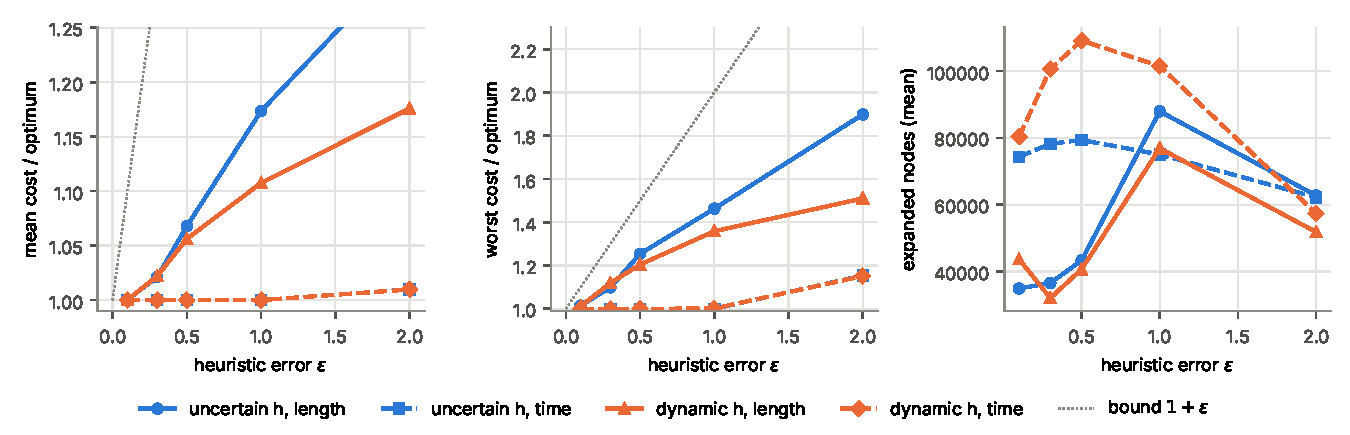
\includegraphics[width=\linewidth]{figures/fig2_eps.pdf}
\caption{Part 1: quality and effort of the inexact heuristics as the error
$\varepsilon$ grows (Platform~C). Dotted line: the guaranteed bound.}
\label{fig:eps}
\end{figure}

\textbf{The loss stays far below the bound.} Up to $\varepsilon=0.3$ the mean
loss is about 2\,\% and the worst case is 9.9\,\% (uncertain) and 11.9\,\%
(dynamic), against a guaranteed 30\,\%. Even at $\varepsilon=2$ the worst
route is 1.90$\times$ the optimum, not 3$\times$. The guarantee is
pessimistic because the error only hurts when the heuristic over-estimates on
the nodes of the optimal path. \textbf{The effort, however, rises sharply.}
Re-openings and stale keys cost so much extra work that the inexact searches
always expand more nodes than A* with the exact straight-line heuristic: 36\,539
(uncertain) and 32\,040 (dynamic) at $\varepsilon=0.3$, and 87\,937 at
$\varepsilon=1$, against 25\,806. The dynamic heuristic needs far more lazy
re-keying than the uncertain one (81\,446 against 13\,064 stale pops per query
at $\varepsilon=0.3$), because its error drifts in one direction for hundreds
of expansions. For travel time the loss is smaller still: the time heuristic
is so weak that even a doubled estimate rarely over-estimates (worst case 1.15
at $\varepsilon=2$).

\begin{figure}[H]
\centering
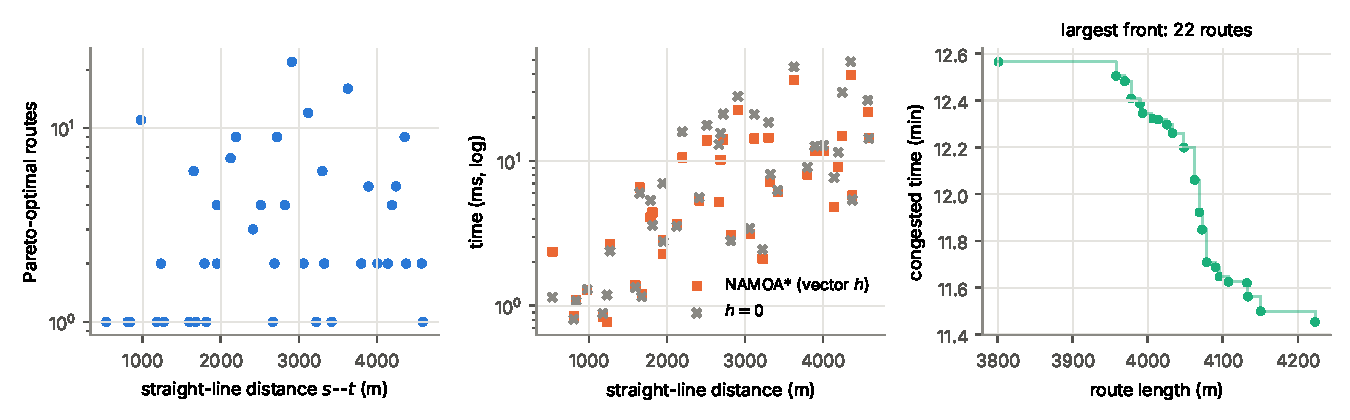
\includegraphics[width=\linewidth]{figures/fig3_namoa.pdf}
\caption{Part 1: \NAMOA{} on 40 queries of increasing distance (Platform~C):
size of the Pareto front (left), run time against the uninformed search with
$h=0$ (middle), and the largest front found (right).}
\label{fig:namoa}
\end{figure}

\textbf{Vector-valued $f$.} The number of Pareto-optimal routes ranges from 1
to 22 (median 2) and depends on the shape of the city between $s$ and $t$ more
than on the distance. When main roads and side streets run parallel, many
trade-offs exist; otherwise one route is best in both objectives. The front
size decides the cost: on Platform~C the query with 22 routes takes 22.6\,ms,
while queries with a single Pareto-optimal route take 0.8--14\,ms. The vector
heuristic makes \NAMOA{} expand $1.7\times$ fewer labels (median) than the
same search with $h=0$, and the exhaustive cross-checks of T5 found no
difference between the two fronts.

\paragraph{Dynamic world: re-planning while driving.} To use A* in a world
that changes, we simulated 40 trips of at least 3.5\,km on the travel-time
metric. Every 15 driven edges, three traffic jams (3--8$\times$ slower, radius
300\,m) appear on the road ahead. Strategy~1 keeps following the initial plan.
Strategy~2 re-plans with A* from the current position after each update; a
jam only increases costs, so the straight-line $h$ stays admissible.

\begin{figure}[H]
\centering
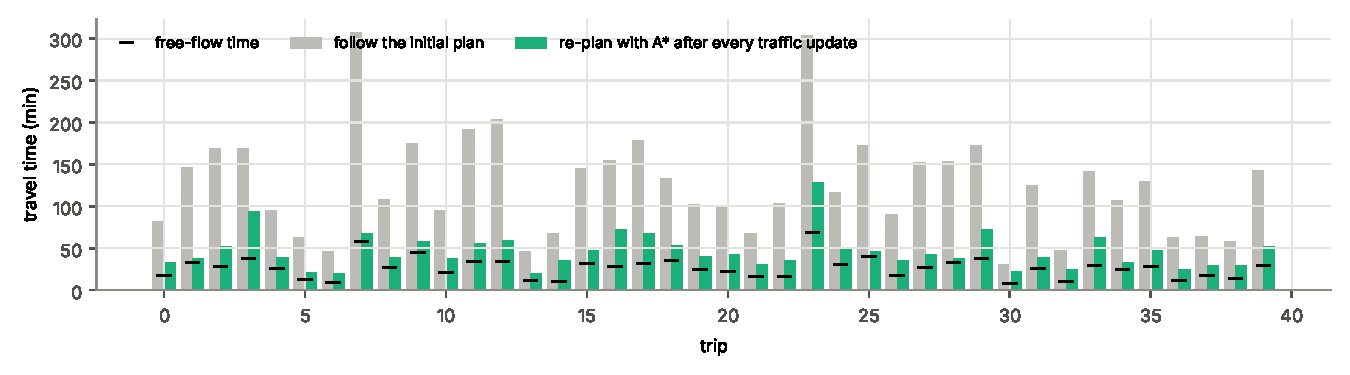
\includegraphics[width=\linewidth]{figures/fig4_dynamic.pdf}
\caption{Part 1: travel time of 40 simulated trips when traffic jams appear
while driving (Platform~C).}
\label{fig:dynamic}
\end{figure}

Re-planning reduces the mean trip from 125.5 to 45.9 minutes (free-flow time
26.6 minutes) and is never worse than following the initial plan. It needs on
average 16.5 re-plans per trip of 16.5\,ms each on Platform~C (6.0\,ms on B),
which is fast enough to run on every traffic update.
